%% LyX 2.0.6 created this file.  For more info, see http://www.lyx.org/.
%% Do not edit unless you really know what you are doing.
\documentclass{article}\usepackage[]{graphicx}\usepackage[]{color}
%% maxwidth is the original width if it is less than linewidth
%% otherwise use linewidth (to make sure the graphics do not exceed the margin)
\makeatletter
\def\maxwidth{ %
  \ifdim\Gin@nat@width>\linewidth
    \linewidth
  \else
    \Gin@nat@width
  \fi
}
\makeatother

\definecolor{fgcolor}{rgb}{0.345, 0.345, 0.345}
\newcommand{\hlnum}[1]{\textcolor[rgb]{0.686,0.059,0.569}{#1}}%
\newcommand{\hlstr}[1]{\textcolor[rgb]{0.192,0.494,0.8}{#1}}%
\newcommand{\hlcom}[1]{\textcolor[rgb]{0.678,0.584,0.686}{\textit{#1}}}%
\newcommand{\hlopt}[1]{\textcolor[rgb]{0,0,0}{#1}}%
\newcommand{\hlstd}[1]{\textcolor[rgb]{0.345,0.345,0.345}{#1}}%
\newcommand{\hlkwa}[1]{\textcolor[rgb]{0.161,0.373,0.58}{\textbf{#1}}}%
\newcommand{\hlkwb}[1]{\textcolor[rgb]{0.69,0.353,0.396}{#1}}%
\newcommand{\hlkwc}[1]{\textcolor[rgb]{0.333,0.667,0.333}{#1}}%
\newcommand{\hlkwd}[1]{\textcolor[rgb]{0.737,0.353,0.396}{\textbf{#1}}}%

\usepackage{framed}
\makeatletter
\newenvironment{kframe}{%
 \def\at@end@of@kframe{}%
 \ifinner\ifhmode%
  \def\at@end@of@kframe{\end{minipage}}%
  \begin{minipage}{\columnwidth}%
 \fi\fi%
 \def\FrameCommand##1{\hskip\@totalleftmargin \hskip-\fboxsep
 \colorbox{shadecolor}{##1}\hskip-\fboxsep
     % There is no \\@totalrightmargin, so:
     \hskip-\linewidth \hskip-\@totalleftmargin \hskip\columnwidth}%
 \MakeFramed {\advance\hsize-\width
   \@totalleftmargin\z@ \linewidth\hsize
   \@setminipage}}%
 {\par\unskip\endMakeFramed%
 \at@end@of@kframe}
\makeatother

\definecolor{shadecolor}{rgb}{.97, .97, .97}
\definecolor{messagecolor}{rgb}{0, 0, 0}
\definecolor{warningcolor}{rgb}{1, 0, 1}
\definecolor{errorcolor}{rgb}{1, 0, 0}
\newenvironment{knitrout}{}{} % an empty environment to be redefined in TeX

\usepackage{alltt}

\usepackage{mathpazo}
\renewcommand{\sfdefault}{lmss}
\renewcommand{\ttdefault}{lmtt}
\usepackage[T1]{fontenc}
\usepackage{geometry}
\geometry{verbose,tmargin=2.5cm,bmargin=2.5cm,lmargin=2.5cm,rmargin=2.5cm}
\usepackage{setspace}
\onehalfspacing
\usepackage{url}
\usepackage{xspace}
\usepackage{multicol}
\usepackage[backend=bibtex, sorting=none]{biblatex}
\usepackage{lineno}
%\usepackage[authoryear]{natbib}
\usepackage{hyperref}
\bibliography{references}

\makeatletter
%%%%%%%%%%%%%%%%%%%%%%%%%%%%%% User specified LaTeX commands.
% \VignetteIndexEntry{An Introduction to knitr}
% \VignetteEngine{knitr::knitr}
\newcommand{\pkg}[1]{{\fontseries{b}\selectfont #1}}
\renewcommand{\pkg}[1]{{\textsf{#1}}}

\newcommand{\code}[1]{\texttt{#1}}

\newcommand{\note}[1]{\textcolor{cyan}{\textbf{#1}}\xspace}

\newcommand{\analyst}{\textit{analyst}\xspace}
\newcommand{\developer}{\textit{developer}\xspace}

\makeatother
\IfFileExists{upquote.sty}{\usepackage{upquote}}{}
\begin{document}
\linenumbers



\title{An Introduction to one-class classification with the \pkg{oneClass} Package}
\author{Benjamin Mack}
\maketitle
\tableofcontents

\newpage

\section{One-class classification}
% A purpose of a one-class classifier is the same than the one of a binary classifier. 
% It is used to classify unknown data samples (e.g. pixels of a remote sensing image)
% to one of two classes. 
% In the case of one-class classification these two classes are often termed positive/negative, presence/absence, or class of interest/rest. 
% In both cases the classification models are learned from data but with an important difference. 
% A binary classification model is trained with labeled data of both classes, and eventually unlabeled data.
% Insted, a one-class classifier is trained with labele data of one class only 

The purpose of \textbf{one-class classifier} is identical to the to classify new data based on a 
classification model learned from labeled examples.
For the training of the classifier labeled samples are only required for the 
positive class, i.e. the class of interest.
Here is the difference to a binary classifier which has to be trained with
labeled data of both the positive and the negative class.
Thus, a one-class classifier is employed when the acquisition of 
representative labeled data for the negative class is expensive or not possible 
at all. 

The convenience of not requiring negative training data comes at a price
because OCC challenging due to the limited information contained in the training 
set.
Unlabeled training data can, and usually should, be used to build more accurate
predictive models. 
However, the process is still uncertain and the classification outcome has to be 
treated with caution. 

\note{A paragraph about the importance of model selection, the difficulty when 
only PU-data is available, about resampling and performance metrics ... .}

The package \pkg{oneClass} shall serve the requirements of \textbf{two potential 
users}, the \analyst and the \developer. These are extrem characters and in 
reality one will usually be located somewhere in between.

The \textbf{\analyst} is faced with a particular one-class classification 
problem, i.e. a set of positive training samples and the unlabeled data to be 
classified.
It is assumed that no complete and representative test set is 
available for the purpose of validation and testing.
In such a situation a careful evaluation of the classification outcome based on 
the available (positive and unlabeled) data is required in order to select the 
most promising final model. 
In section\ref{sec:analyst} the analysis strategy presented in 
\note{REF} is followed and the main functions are illustrated.
Hopefully the package can be helpful to solve a given one-class classification 
problem more effective and more convenient in practice. 

The \textbf{\developer} is interested in the developement of new and/or optimization of 
existing methods. Therefore the package provides convenient functionalities.
The package \pkg{oneClass} builds upon the powerful package \pkg{caret} \cite{Kuhn.2014} and tries
to adapt the philosophy. 

The package \pkg{caret} allows one to embed own \textbf{custom functionalities} in the 
rich infrastructure of the \pkg{caret} package, in fact the one-class classification
methods of the \package{oneClass} are implemented as custom functions which are passed 
to the function \hlkwd{train}\hlstd{()}. 
This infrastructure comprises  methods for pre-processing data, calculating 
variable importance, model visualizations, and parallel processing. 

The function \hlkwd{oneClass}\hlstd{()} calls the \hlstd{caret::}\hlkwd{train}\hlstd{()} 
function with a one-class methods. It returns an object of class \code{oneClass}
which inherits from the class \code{train}. Thus, many of the powerful analysis 
tools from the train package can also be used seemlessly when using an object of 
class \code{oneClass}.

\subsubsection*{One-class classifiers}

The \pkg{oneClass} package is a user-oriented environment for analyzing 
one-class classification problems.
It implements two commonly used classifiers, the biased SVM \cite{BingLiu.2002, Liu.2003}, and Maxent \cite{Elith.2011, Phillips.2008b}. 

These classifiers are implemented as costum functions for the 
\hlkwd{train}\hlstd{()} function from the \pkg{caret} package \note{[REF]}.
Thus the extensive functionalitie of \hlkwd{train}\hlstd{()} can be used for model selection.

\subsubsection*{PU-performance metrics}

...

\section{Installation}
\label{sec:installation}

Currently the package is still not on R CRAN but can be downloaded from GitHub 
(\url{https://github.com/benmack/oneClass}).
It can be installed in R with the package \code{devtools} and the following commands (This may take a while...):

\begin{knitrout}
\definecolor{shadecolor}{rgb}{0.969, 0.969, 0.969}\color{fgcolor}\begin{kframe}
\begin{alltt}
\hlkwd{library}\hlstd{(devtools)}
\hlkwd{install_github}\hlstd{(}\hlstr{'benmack/oneClass'}\hlstd{)}
\end{alltt}
\end{kframe}
\end{knitrout}

\section{Synthetic data: bananas}
\label{sec:data}


In the following the package is demonstrated by means of the synthetic banana data set 
which is included in the package. 

The \hlstd{bananas} data is stored as \hlstd{raster} data, where \hlstd{y} is a one-band raster with the class patches, i.e. what we want to find out when performing one-class classification with remotely sensed data. 
\hlstd{x} are the features or predictors based on which the classification has to be build. 

\begin{knitrout}
\definecolor{shadecolor}{rgb}{0.969, 0.969, 0.969}\color{fgcolor}\begin{kframe}
\begin{alltt}
\hlkwd{require}\hlstd{(oneClass)}
\hlkwd{require}\hlstd{(raster)}
\hlkwd{data}\hlstd{(bananas)}
\hlkwd{plot}\hlstd{(}\hlkwd{stack}\hlstd{(bananas}\hlopt{$}\hlstd{y, bananas}\hlopt{$}\hlstd{x),} \hlkwc{nc}\hlstd{=}\hlnum{3}\hlstd{)}
\end{alltt}
\end{kframe}
\end{knitrout}

\begin{knitrout}
\definecolor{shadecolor}{rgb}{0.969, 0.969, 0.969}\color{fgcolor}\begin{figure}[]


{\centering 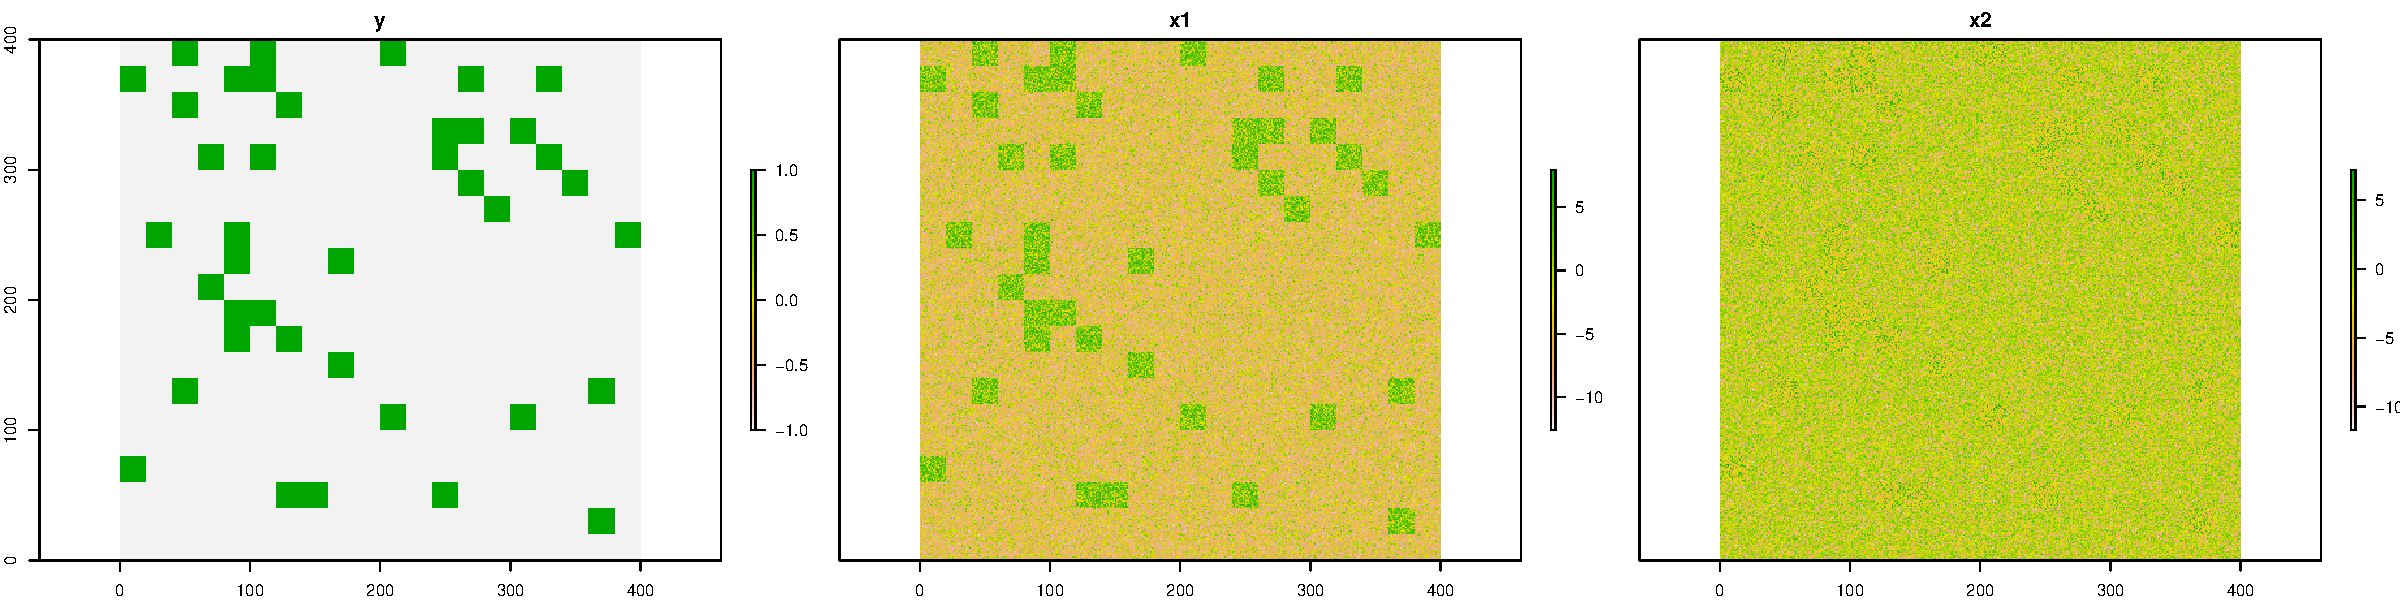
\includegraphics[width=\maxwidth]{figures/plots-loadpkg_prelim} 

}

\caption[The class membership (left), and the two features (middle and right) of the synthetic bananas data set]{The class membership (left), and the two features (middle and right) of the synthetic bananas data set.\label{fig:loadpkg_prelim}}
\end{figure}


\end{knitrout}

In one-class classification a set of positive labeled samples is available for 
training the classifier.
Furthermore, unlabeled samples are used, which are usually a random sample of the
whole data.
Such a training data set is also stored in the bananas data set. 
Additionally we generate a test data set consisting of 1.000 random samples of the 
image. 
As we mentioned before, we would not expect to have a test set in real-world 
one-class classification application. 
But here we also create a PN test data set (PN-data) to show the available 
(PN-) evaluation methods which are useful when investigating one-class classifiers 
of developing new methods.

\begin{knitrout}
\definecolor{shadecolor}{rgb}{0.969, 0.969, 0.969}\color{fgcolor}\begin{kframe}
\begin{alltt}
\hlstd{seed} \hlkwb{<-} \hlnum{123456}
\hlstd{tr.x} \hlkwb{<-} \hlstd{bananas}\hlopt{$}\hlstd{tr[,} \hlopt{-}\hlnum{1}\hlstd{]}
\hlstd{tr.y} \hlkwb{<-} \hlkwd{puFactor}\hlstd{(bananas}\hlopt{$}\hlstd{tr[,} \hlnum{1}\hlstd{],} \hlkwc{positive}\hlstd{=}\hlnum{1}\hlstd{)}
\hlkwd{set.seed}\hlstd{(seed)}
\hlstd{te.i} \hlkwb{<-} \hlkwd{sample}\hlstd{(}\hlkwd{ncell}\hlstd{(bananas}\hlopt{$}\hlstd{y),} \hlnum{1000}\hlstd{)}
\hlstd{te.x} \hlkwb{<-} \hlkwd{extract}\hlstd{(bananas}\hlopt{$}\hlstd{x, te.i)}
\hlstd{te.y} \hlkwb{<-} \hlkwd{extract}\hlstd{(bananas}\hlopt{$}\hlstd{y, te.i)}
\end{alltt}
\end{kframe}
\end{knitrout}


With the two-dimensional synthetic data set we can view the data in the feature 
space:

\begin{knitrout}
\definecolor{shadecolor}{rgb}{0.969, 0.969, 0.969}\color{fgcolor}\begin{kframe}
\begin{alltt}
\hlkwd{par}\hlstd{(}\hlkwc{mfrow}\hlstd{=}\hlkwd{c}\hlstd{(}\hlnum{1}\hlstd{,}\hlnum{2}\hlstd{),} \hlkwc{mgp}\hlstd{=}\hlkwd{c}\hlstd{(}\hlnum{1.75}\hlstd{,} \hlnum{.75}\hlstd{,} \hlnum{0}\hlstd{),} \hlkwc{mar}\hlstd{=}\hlkwd{c}\hlstd{(}\hlnum{3}\hlstd{,} \hlnum{3}\hlstd{,} \hlnum{.1}\hlstd{,} \hlnum{.1}\hlstd{))}
\hlkwd{plot}\hlstd{(tr.x,} \hlkwc{pch}\hlstd{=}\hlkwd{ifelse}\hlstd{(tr.y}\hlopt{==}\hlnum{1}\hlstd{,} \hlnum{16}\hlstd{,} \hlnum{4}\hlstd{) )}
\hlkwd{plot}\hlstd{(te.x,} \hlkwc{pch}\hlstd{=}\hlkwd{ifelse}\hlstd{(te.y}\hlopt{==}\hlnum{1}\hlstd{,} \hlnum{16}\hlstd{,} \hlnum{4}\hlstd{) )}
\end{alltt}
\end{kframe}

{\centering 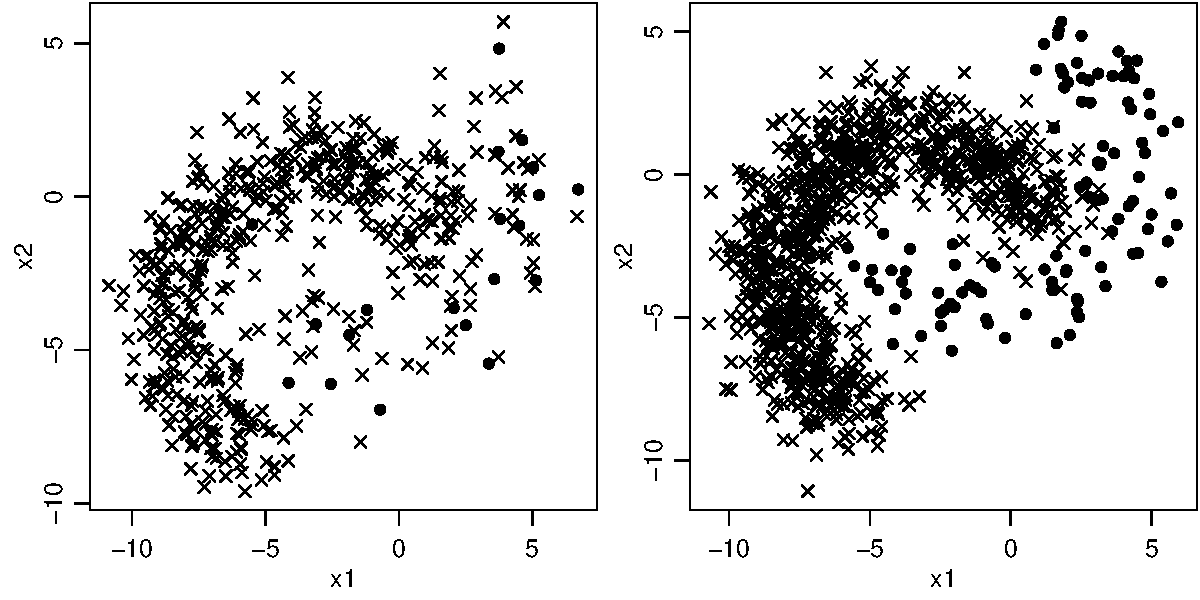
\includegraphics[width=0.8\textwidth]{figures/plots-featurespace_trainTest} 

}



\end{knitrout}

A one-class classifier is supposed to learn from the PU-data (left) to optimally 
classify the PN data (right).

\section{Model selection in the absence of PN-data.}
\label{sec:analyst}

\hlkwd{oneClass}\hlstd{()} requires the training data as input.
We also pass the whole unlabeled data because we want to analyze the predicted 
outcome of the whole data to better examine the performance of the model.  
Of course, if the data is very large, it is possible to use a subset here. 



\begin{knitrout}
\definecolor{shadecolor}{rgb}{0.969, 0.969, 0.969}\color{fgcolor}\begin{kframe}
\begin{alltt}
\hlkwd{set.seed}\hlstd{(seed)}
\hlstd{index} \hlkwb{<-} \hlkwd{createFolds}\hlstd{( tr.y,} \hlkwc{k}\hlstd{=}\hlnum{10}\hlstd{,} \hlkwc{returnTrain}\hlstd{=}\hlnum{TRUE} \hlstd{)}
\hlstd{trControl} \hlkwb{<-} \hlkwd{trainControl}\hlstd{(}\hlkwc{method}\hlstd{=}\hlstr{'cv'}\hlstd{,}
                          \hlkwc{index}\hlstd{=index,}
                          \hlkwc{summaryFunction} \hlstd{= puSummary,}  \hlcom{# PU-performance metrics}
                          \hlkwc{classProbs}\hlstd{=}\hlnum{TRUE}\hlstd{,}              \hlcom{# important }
                          \hlkwc{savePredictions} \hlstd{=} \hlnum{TRUE}\hlstd{,}       \hlcom{# important}
                          \hlkwc{returnResamp} \hlstd{=} \hlstr{'all'}\hlstd{)}         \hlcom{# for resamples.train }
\hlstd{oc} \hlkwb{<-} \hlkwd{oneClass}\hlstd{(} \hlkwc{x} \hlstd{= tr.x,} \hlkwc{y} \hlstd{= tr.y,} \hlkwc{trControl} \hlstd{= trControl )}
\hlstd{pred} \hlkwb{<-} \hlkwd{predict}\hlstd{(oc, bananas}\hlopt{$}\hlstd{x)}
\end{alltt}
\end{kframe}
\end{knitrout}

In a later section the internal processing steps of \hlkwd{oneClass}\hlstd{()} are 
explained in more detail.
Now we want to understand if the trained model is reasonable. 
The distributions of the predicted training data (\hlstd{tr.x}) and unlabeled 
data (\code{bananas\$x}) can help to make a first diagnosis. 
They are figures in the left plot below which we refer to as the 'diagnostic plot' (histogram: predicted unlabeled data, blue/grey boxplots: held-out predictions of the positive/unlabeled training samples).
The right plot shows the model, i.e. the separating hyperplane of the biased SVM model (black line)
and the distances (color coded). 
Please note that the color code in the right plot corresponds to the x-axis in the left plot. 

Of course, in practice the right plot can not be visualized because the input data 
space is usually high dimensional. 
We show it here to facilitate the understanding of the interpretation.

\begin{knitrout}
\definecolor{shadecolor}{rgb}{0.969, 0.969, 0.969}\color{fgcolor}\begin{kframe}
\begin{alltt}
\hlkwd{plot}\hlstd{(pred)}
\hlkwd{hist}\hlstd{(oc, pred)}
\hlkwd{featurespace}\hlstd{(oc,} \hlkwc{th}\hlstd{=}\hlnum{0}\hlstd{)}
\end{alltt}
\end{kframe}
\end{knitrout}


\begin{multicols}{3}
\begin{knitrout}
\definecolor{shadecolor}{rgb}{0.969, 0.969, 0.969}\color{fgcolor}

{\centering 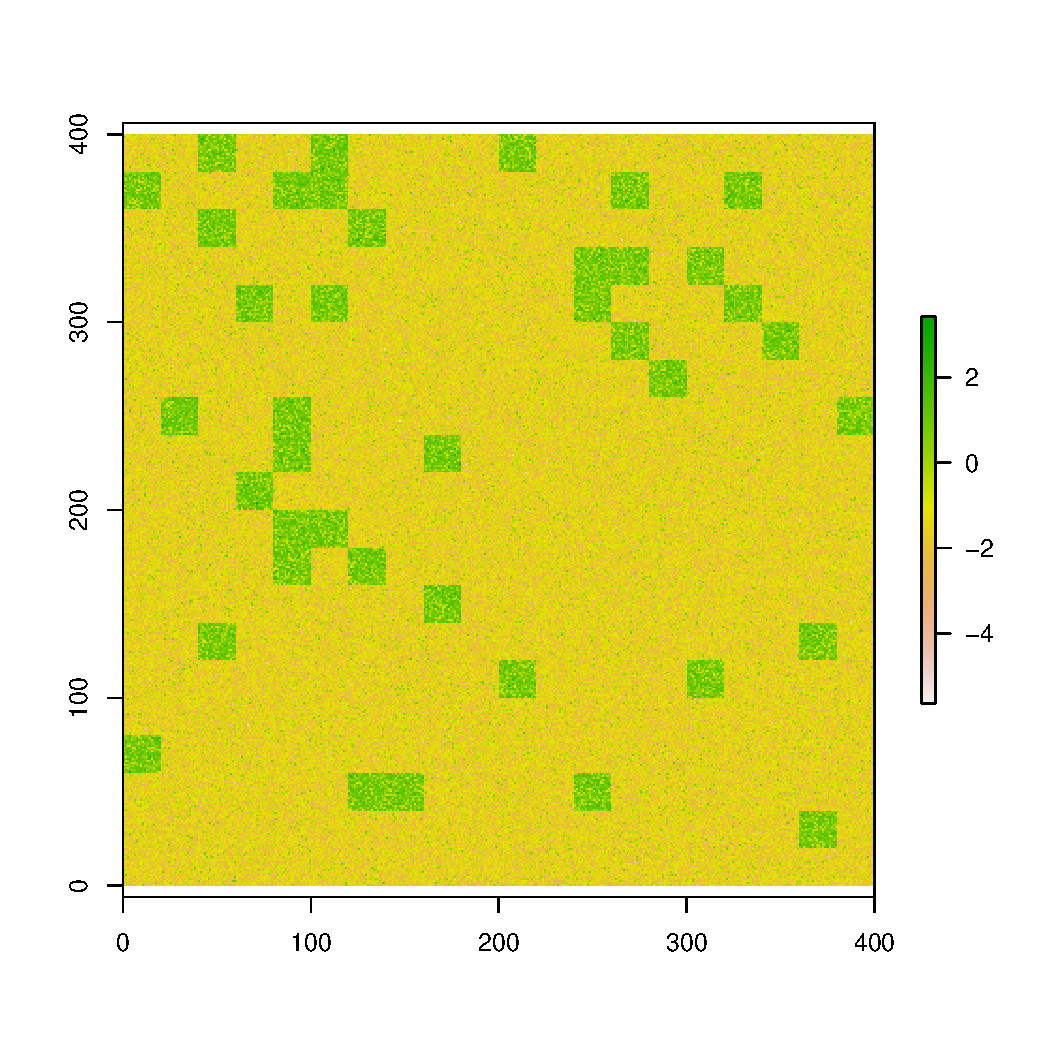
\includegraphics[width=.95\linewidth]{figures/plots-img_plot} 

}



\end{knitrout}

\begin{knitrout}
\definecolor{shadecolor}{rgb}{0.969, 0.969, 0.969}\color{fgcolor}

{\centering 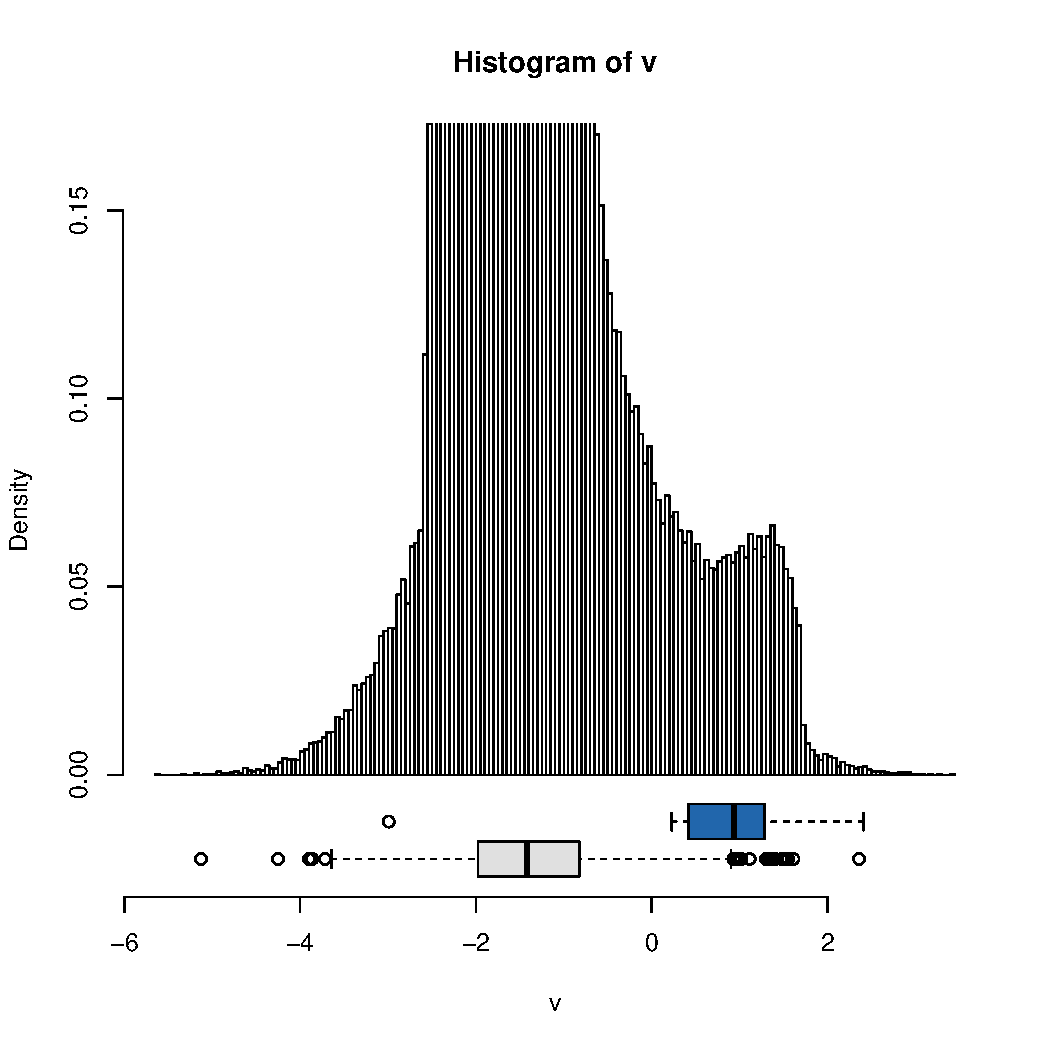
\includegraphics[width=.95\linewidth]{figures/plots-hist_plot} 

}



\end{knitrout}

\begin{knitrout}
\definecolor{shadecolor}{rgb}{0.969, 0.969, 0.969}\color{fgcolor}

{\centering 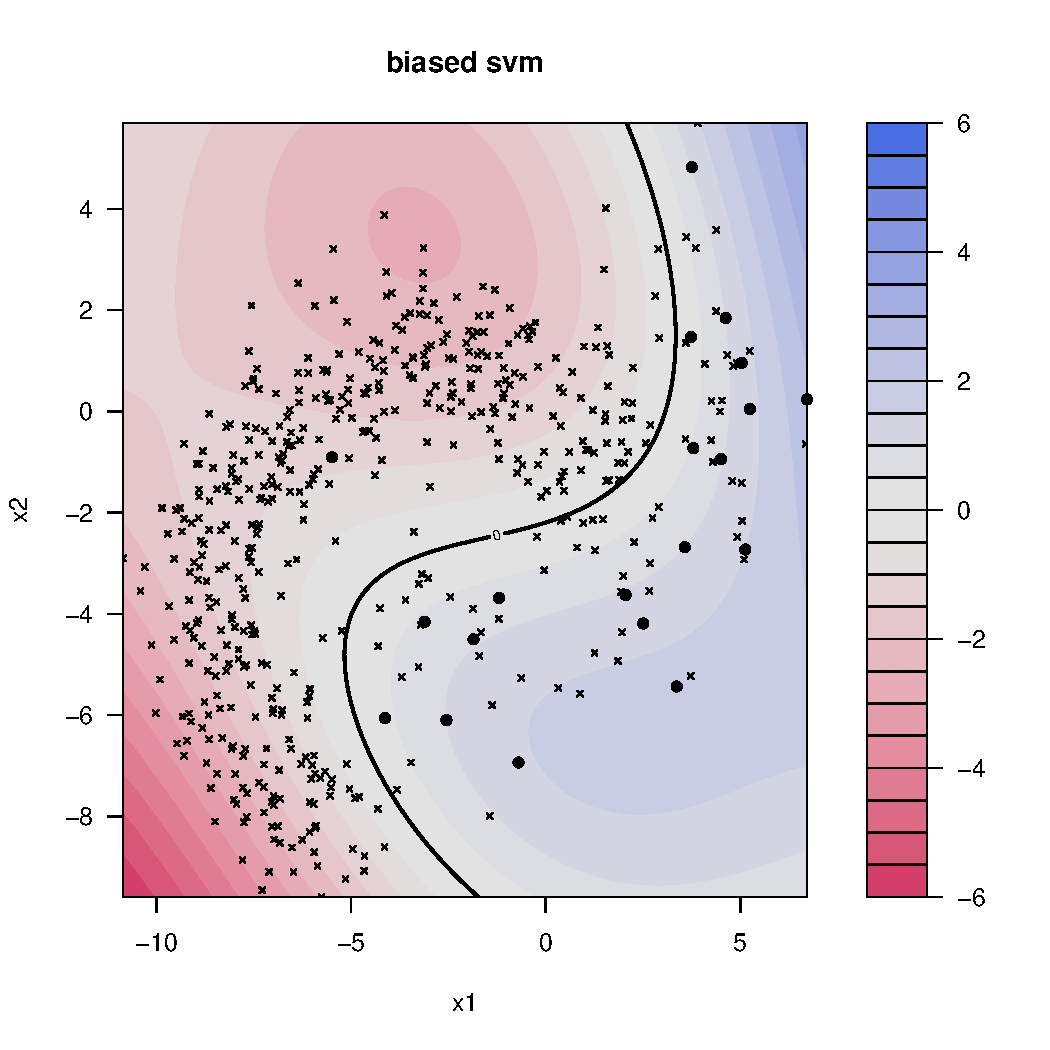
\includegraphics[width=.95\linewidth]{figures/plots-featurespace_plot} 

}



\end{knitrout}
\end{multicols}

From the diagnostic plot important conclusions can be derived about the training data, 
the class separability, and the suitability of a threshold for binarization, i.e. 
the conversion of the continuous classifier output in a binary classification. 

In the envisaged strategy, the careful interpretation of the diagnostic plot is 
a critical element of the whole one-class classification processing chain. It 
provides the analyst with information based on which decisions are made.

The interpretation of the diagnostic plot reads as follows:

Regarding the \textbf{training data} we can assume that the amount of unlabeled training data is sufficient.
This is because the positive and unlabeled training data overlaps (recognizable by the boxplots).
This is very important. 
Imagine the complete unlabeled training data would be located at very low predictive values. 
In this case we could not be confident that the the unlableled training contains the relevant 
information required to build the model. 
Of course, if the data is well separable and/or the optimal decision boundary is very complex (non-linear) it is still possible to derive a good classifier. 
However, if this is not the case, the model is likely to be biased and/or to underfit the data. 

Regarding the \textbf{separability} the following conclusions can be made:\\
The positive training data corresponds well with a distinctive cluster of data in the histogram at high predictive values.
This cluster is separated by a low density area from the rest of the majority of the data.
If we assume that the positive data set is representative and sufficiently large for the positive class we can conclude that the classification model is suitable and has a high discriminative power.

Regarding the \textbf{suitability of the threshold} we can assume that any threshold in the low density region leads to relatively high accuracies. 

Nevertheless, it is always a good idea to examine the relationship between the estimated PU-performance and the tuneing parameters.
\pkt{caret} offers different ploting functions for this purpose \footnote{\url{http://caret.r-forge.r-project.org/training.html}}. 
For example, here the \code{puF} and \code{puAuc} performance metrics are plotted in a heatmap.

\begin{knitrout}
\definecolor{shadecolor}{rgb}{0.969, 0.969, 0.969}\color{fgcolor}\begin{kframe}
\begin{alltt}
\hlkwd{trellis.par.set}\hlstd{(}\hlkwd{caretTheme}\hlstd{())} \hlcom{# nice colors from caret}
\hlkwd{plot}\hlstd{(oc,} \hlkwc{metric} \hlstd{=} \hlstr{'puF'}\hlstd{,} \hlkwc{plotType} \hlstd{=} \hlstr{"level"}\hlstd{)}
\hlkwd{plot}\hlstd{(oc,} \hlkwc{metric} \hlstd{=} \hlstr{'puAuc'}\hlstd{,} \hlkwc{plotType} \hlstd{=} \hlstr{"level"}\hlstd{)}
\end{alltt}
\end{kframe}

{\centering 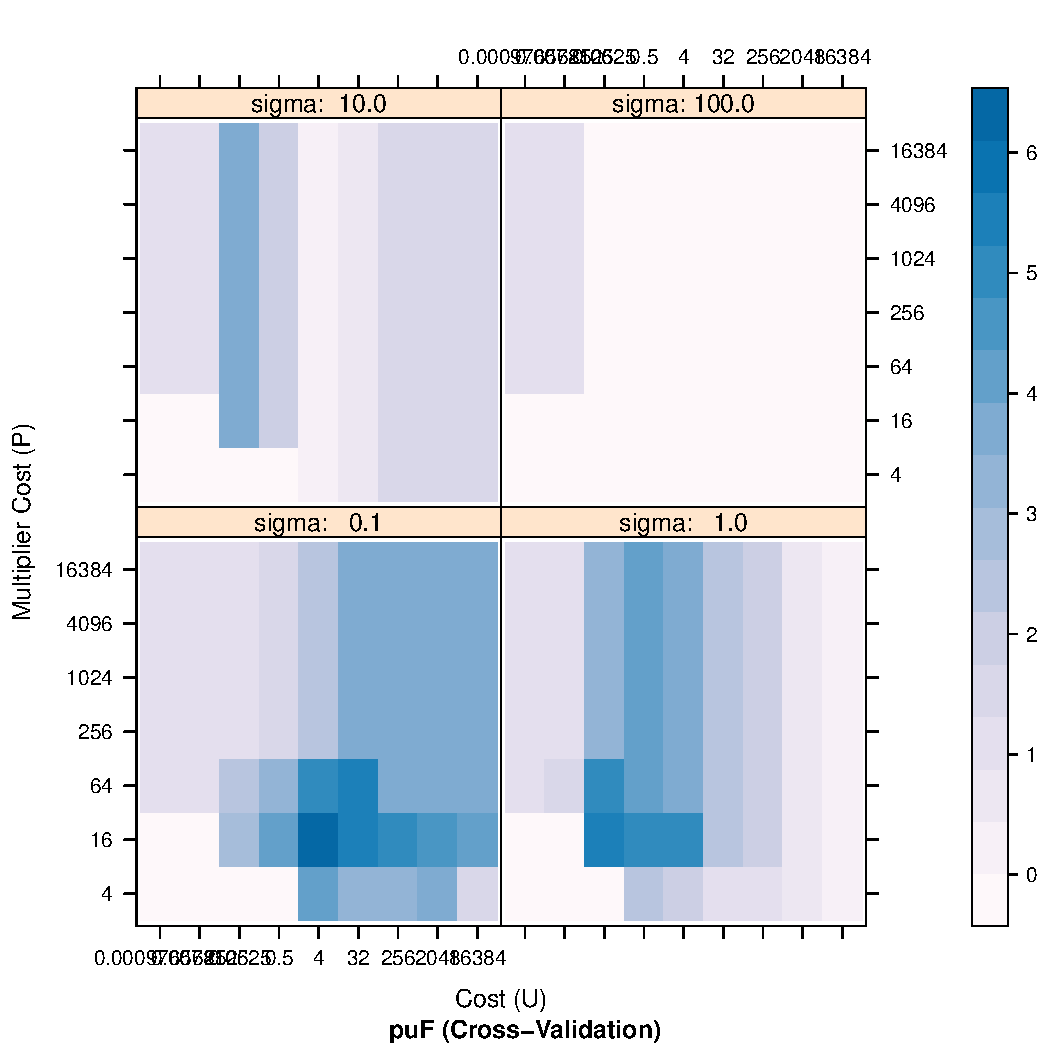
\includegraphics[width=.5\textwidth]{figures/plots-levelplots1} 
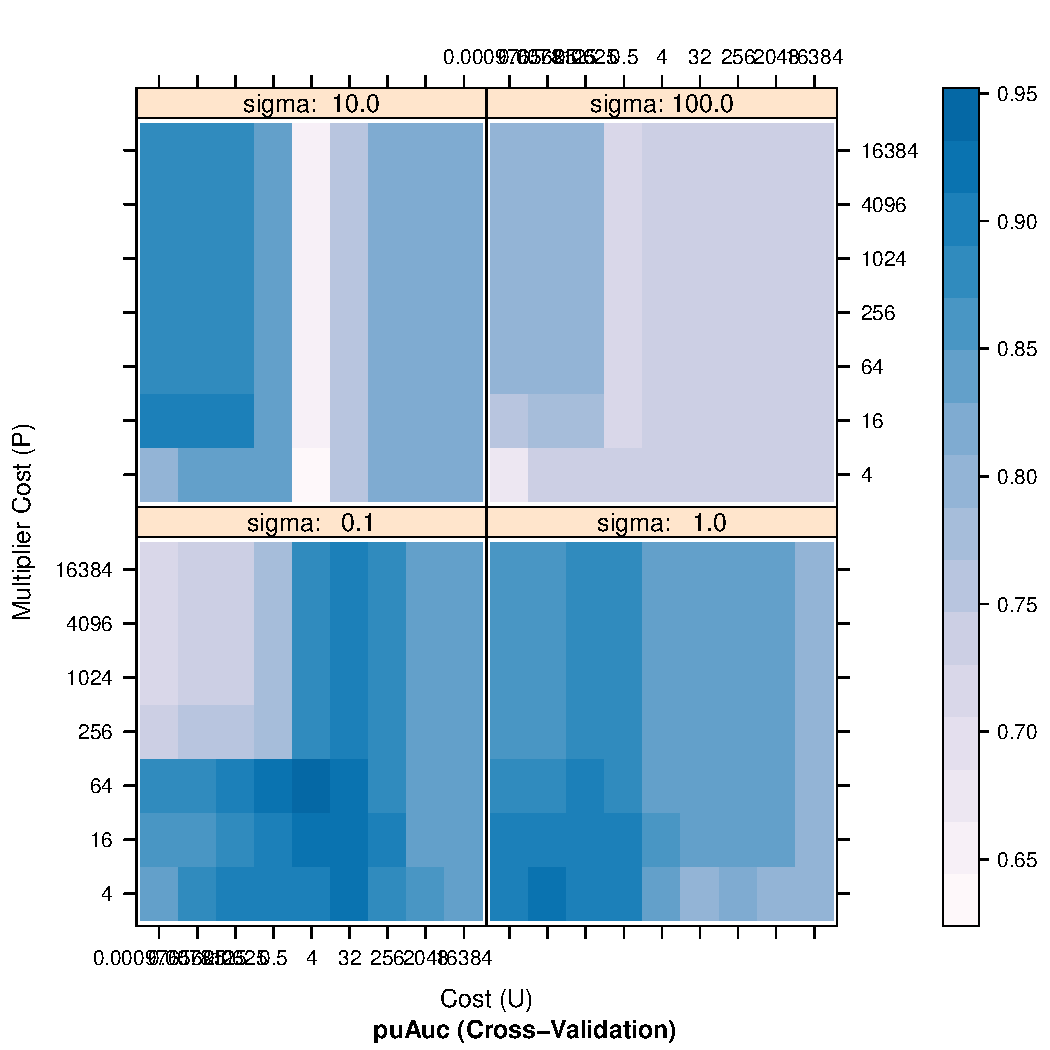
\includegraphics[width=.5\textwidth]{figures/plots-levelplots2} 

}



\end{knitrout}

These plots are informative to evaluate the tuning process and the final model. 
First, we can see if the parameter space in which we were looking for the optimal model has been reasonable. 
In the case here this is true because the models with the highest PU-performances are not located at the border of the parameter space. 
If this would be the case, a moor suitable parameter combination could possibly lead to more powerful model.
Also in the case where the optimal models are located at intermedate parameter values it is possible to find better models by repeating the model tuning over a finer grid of parameters in the space of optimal models. 
This is particularly recommendable if the estimated performance does not change smoothly with the parameters.  

We can also examine the table which is printed when printing an object of class \code{train} or its inheriting child \code{oneClass}.
Here we do not print the full table, as it is too large but an ordered and subsetted version 
of the complete table.

\begin{knitrout}\footnotesize
\definecolor{shadecolor}{rgb}{0.969, 0.969, 0.969}\color{fgcolor}\begin{kframe}
\begin{alltt}
\hlcom{# oc # --> prints the whole large table with performance metrics of all models}
\hlkwd{sort}\hlstd{(oc,} \hlkwc{printTable}\hlstd{=}\hlnum{TRUE}\hlstd{,} \hlkwc{rows}\hlstd{=}\hlnum{1}\hlopt{:}\hlnum{10}\hlstd{,} \hlkwc{by}\hlstd{=}\hlstr{'puF'}\hlstd{,} \hlkwc{digits}\hlstd{=}\hlnum{2}\hlstd{)}
\end{alltt}
\begin{verbatim}
##    sigma    cNeg cMultiplier puAuc puF  Tpr puPpv puAucSD puFSD TprSD puPpvSD
## 30   0.1 4.0e+00          16  0.92 6.1 0.95  0.16   0.107   2.1  0.16   0.040
## 38   0.1 3.2e+01          64  0.92 5.4 0.90  0.16   0.091   2.1  0.21   0.054
## 37   0.1 3.2e+01          16  0.91 5.4 0.85  0.15   0.117   2.8  0.24   0.044
## 79   1.0 6.2e-02          16  0.91 5.3 0.90  0.16   0.082   2.1  0.21   0.041
## 80   1.0 6.2e-02          64  0.91 5.1 0.95  0.19   0.086   1.8  0.16   0.049
## 86   1.0 5.0e-01          16  0.90 5.1 0.85  0.15   0.099   2.0  0.24   0.043
## 93   1.0 4.0e+00          16  0.85 5.0 0.65  0.12   0.154   3.9  0.41   0.032
## 31   0.1 4.0e+00          64  0.93 4.9 0.95  0.20   0.090   2.0  0.16   0.060
## 44   0.1 2.6e+02          16  0.89 4.8 0.80  0.14   0.117   2.4  0.26   0.049
## 51   0.1 2.0e+03          16  0.85 4.4 0.65  0.13   0.144   2.9  0.41   0.047
\end{verbatim}
\end{kframe}
\end{knitrout}

\begin{knitrout}\footnotesize
\definecolor{shadecolor}{rgb}{0.969, 0.969, 0.969}\color{fgcolor}\begin{kframe}
\begin{alltt}
\hlkwd{sort}\hlstd{(oc,} \hlkwc{printTable}\hlstd{=}\hlnum{TRUE}\hlstd{,} \hlkwc{rows}\hlstd{=}\hlnum{1}\hlopt{:}\hlnum{10}\hlstd{,} \hlkwc{by}\hlstd{=}\hlstr{'puAuc'}\hlstd{,} \hlkwc{digits}\hlstd{=}\hlnum{2}\hlstd{)}
\end{alltt}
\begin{verbatim}
##    sigma    cNeg cMultiplier puAuc puF  Tpr puPpv puAucSD puFSD TprSD puPpvSD
## 31   0.1  4.0000          64  0.93 4.9 0.95 0.204   0.090   2.0  0.16   0.060
## 30   0.1  4.0000          16  0.92 6.1 0.95 0.158   0.107   2.1  0.16   0.040
## 38   0.1 32.0000          64  0.92 5.4 0.90 0.160   0.091   2.1  0.21   0.054
## 71   1.0  0.0078           4  0.92 0.0 0.00 0.000   0.050   0.0  0.00   0.000
## 24   0.1  0.5000          64  0.91 3.4 0.95 0.287   0.105   1.4  0.16   0.067
## 36   0.1 32.0000           4  0.91 3.1 0.40 0.071   0.110   2.3  0.32   0.035
## 37   0.1 32.0000          16  0.91 5.4 0.85 0.148   0.117   2.8  0.24   0.044
## 79   1.0  0.0625          16  0.91 5.3 0.90 0.162   0.082   2.1  0.21   0.041
## 78   1.0  0.0625           4  0.91 0.0 0.00 0.000   0.065   0.0  0.00   0.000
## 80   1.0  0.0625          64  0.91 5.1 0.95 0.188   0.086   1.8  0.16   0.049
\end{verbatim}
\end{kframe}
\end{knitrout}

Thus, according to the \code{puF}-performance metric the model with the parameters
\code{sigma}=0.1, \code{cNeg}=100, and \code{cMultiplier}=8 is the best.
But other models are close behind the metric. 
Furthermore, there are other performance metrics, e.g. the \code{puAuc} which do not
agree with the ranking of the \code{puF}.

It is difficult to say which metric is better. 
They both have different characteristics. 
The f1Pu is a measure which only evaluates at the default threshold 0. 
Thus, even models with high discriminative power can be placed at a low rank when 
the threshold 0 is unsuitable. 
The puAuc instead measures the discriminative over the whole range of possible threshold values. 
However, this can also introduce misleading measures, due to the fact that 
thresholds influence the measure which are far from beeing rational choices \textcolor{red}{[REF]}.

% We have seen that there is a positive relationship between the PU-performance metrics and the test accuracy. 
% But that a model with a high PU can also sometimes have low test accuracy. 

Inspectation of the resampling distributions of differnet models can give more evidence on which the model selection can be founded. 
Let us first find ten models which are ranked highest by the \code{puF} and/or the \code{puAuc}. 

\begin{knitrout}
\definecolor{shadecolor}{rgb}{0.969, 0.969, 0.969}\color{fgcolor}\begin{kframe}
\begin{alltt}
\hlstd{puF.ranking}   \hlkwb{<-} \hlkwd{sort} \hlstd{(oc,} \hlkwc{by}\hlstd{=}\hlstr{'puF'}\hlstd{,} \hlkwc{print}\hlstd{=}\hlnum{FALSE}\hlstd{)}
\hlstd{puAuc.ranking} \hlkwb{<-} \hlkwd{sort} \hlstd{(oc,} \hlkwc{by}\hlstd{=}\hlstr{'puAuc'}\hlstd{,} \hlkwc{print}\hlstd{=}\hlnum{FALSE}\hlstd{)}

\hlstd{candidates} \hlkwb{<-} \hlkwd{as.numeric}\hlstd{(}\hlkwd{unique}\hlstd{(}\hlkwd{c}\hlstd{(}\hlkwd{rownames}\hlstd{(puF.ranking),}
                                  \hlkwd{rownames}\hlstd{(puAuc.ranking)) [}
                                    \hlkwd{rep}\hlstd{(}\hlnum{1}\hlopt{:}\hlnum{10}\hlstd{,} \hlkwc{each}\hlstd{=}\hlnum{2}\hlstd{)}\hlopt{+}\hlkwd{rep}\hlstd{(}\hlkwd{c}\hlstd{(}\hlnum{0}\hlstd{,} \hlnum{10}\hlstd{),} \hlnum{10}\hlstd{) ]))}
\hlstd{candidates[}\hlnum{1}\hlopt{:}\hlnum{10}\hlstd{]}
\end{alltt}
\begin{verbatim}
##  [1] 30 23 38 29 37 58 79 87 80 88
\end{verbatim}
\end{kframe}
\end{knitrout}

For these models let us extract the performance metrics of the resamples and 
compare the resampling distributions between the models. 

\begin{knitrout}
\definecolor{shadecolor}{rgb}{0.969, 0.969, 0.969}\color{fgcolor}\begin{kframe}
\begin{alltt}
\hlstd{resamps} \hlkwb{<-} \hlkwd{resamples.train}\hlstd{(oc,} \hlkwc{modParam}\hlstd{=oc}\hlopt{$}\hlstd{results[candidates,}\hlnum{1}\hlopt{:}\hlnum{3}\hlstd{])}
\hlkwd{bwplot}\hlstd{(resamps,} \hlkwc{metric}\hlstd{=}\hlstr{'puF'}\hlstd{)}
\end{alltt}
\end{kframe}
\end{knitrout}

\begin{knitrout}
\definecolor{shadecolor}{rgb}{0.969, 0.969, 0.969}\color{fgcolor}

{\centering 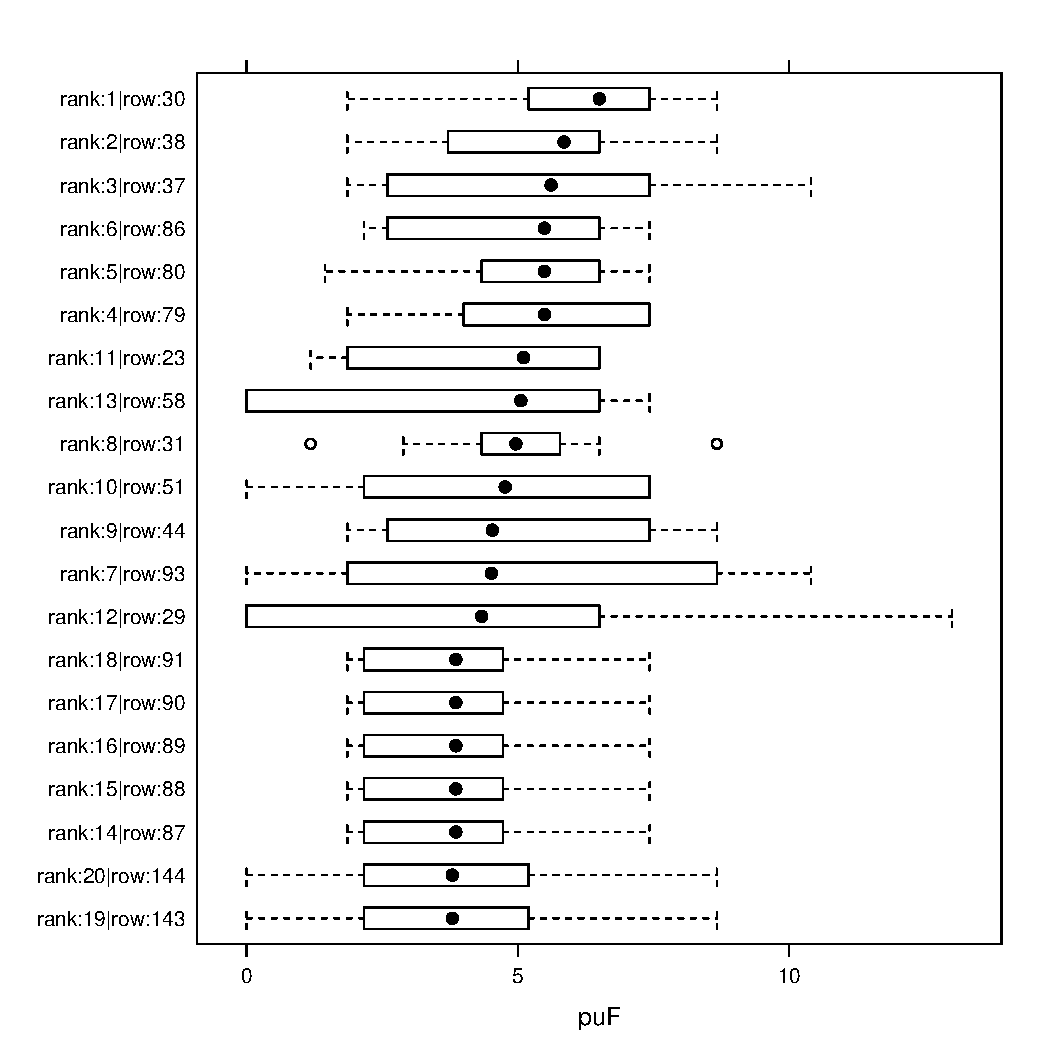
\includegraphics[width=0.75\textwidth]{figures/plots-resamps_eval} 

}



\end{knitrout}

As we can see that the model ranked highest by the \code{puF} measure (second boxplot from the top) has competing models with very similar and resampling distributions. 
These models are not significantly different in terms of the resampling distributions so any one of them is a potential final model. 
It can be helpful to investigate the diagnostic histogram plot of the whole unlabeled data in order to gain more insight in the model characteristics.

\begin{knitrout}
\definecolor{shadecolor}{rgb}{0.969, 0.969, 0.969}\color{fgcolor}\begin{kframe}
\begin{alltt}
\hlstd{oc.candidate1} \hlkwb{<-} \hlkwd{update}\hlstd{(oc,} \hlkwc{u}\hlstd{=bananas}\hlopt{$}\hlstd{x,} \hlkwc{modRow}\hlstd{=candidates[}\hlnum{1}\hlstd{])}
\hlstd{oc.candidate2} \hlkwb{<-} \hlkwd{update}\hlstd{(oc,} \hlkwc{u}\hlstd{=bananas}\hlopt{$}\hlstd{x,} \hlkwc{modRow}\hlstd{=candidates[}\hlnum{2}\hlstd{])}
\hlstd{oc.candidate3} \hlkwb{<-} \hlkwd{update}\hlstd{(oc,} \hlkwc{u}\hlstd{=bananas}\hlopt{$}\hlstd{x,} \hlkwc{modRow}\hlstd{=candidates[}\hlnum{3}\hlstd{])}
\end{alltt}
\end{kframe}
\end{knitrout}


\newpage
\begin{multicols}{3}
\begin{knitrout}
\definecolor{shadecolor}{rgb}{0.969, 0.969, 0.969}\color{fgcolor}

{\centering 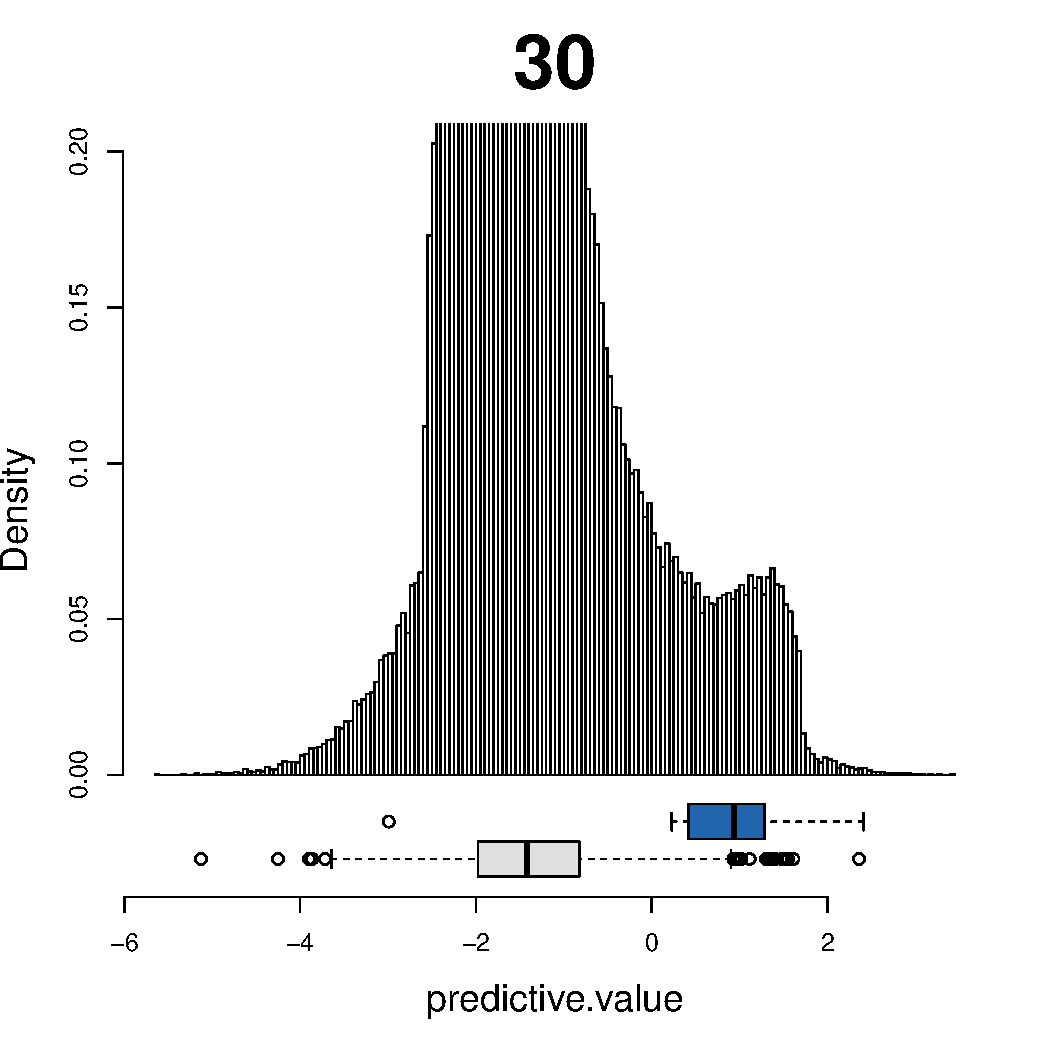
\includegraphics[width=\maxwidth]{figures/plots-update1_hist} 

}



\end{knitrout}

\begin{knitrout}
\definecolor{shadecolor}{rgb}{0.969, 0.969, 0.969}\color{fgcolor}

{\centering 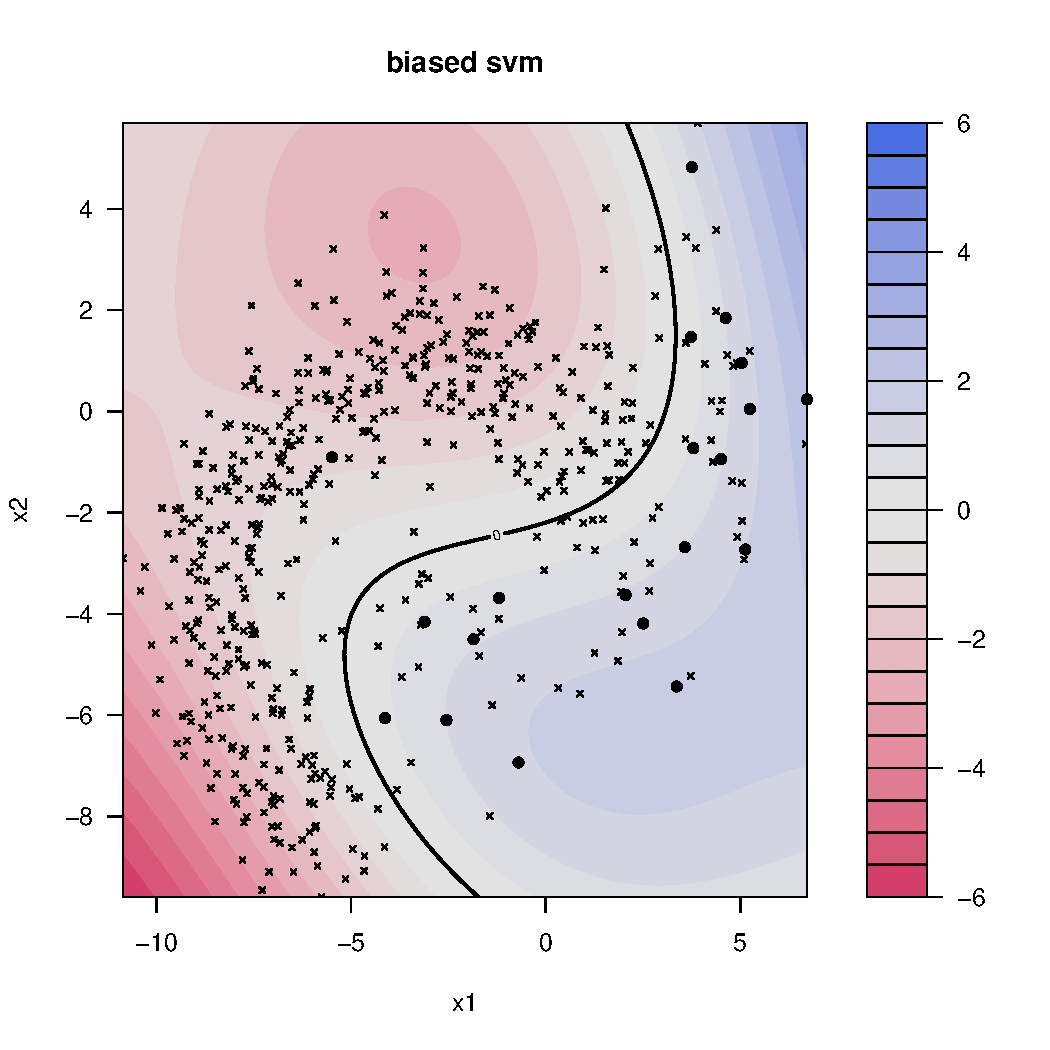
\includegraphics[width=\maxwidth]{figures/plots-update1_fs} 

}



\end{knitrout}

\begin{knitrout}
\definecolor{shadecolor}{rgb}{0.969, 0.969, 0.969}\color{fgcolor}

{\centering 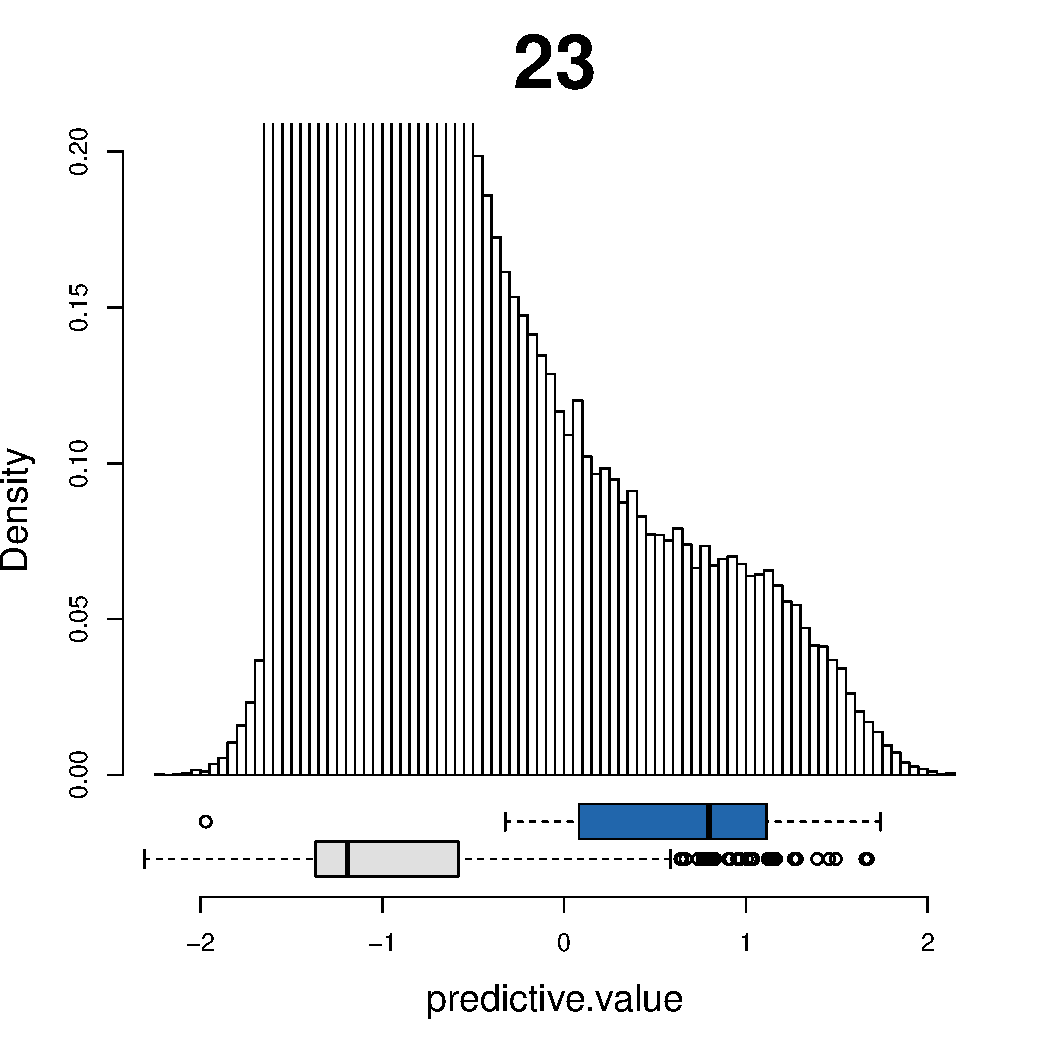
\includegraphics[width=\maxwidth]{figures/plots-update2_hist} 

}



\end{knitrout}

\begin{knitrout}
\definecolor{shadecolor}{rgb}{0.969, 0.969, 0.969}\color{fgcolor}

{\centering 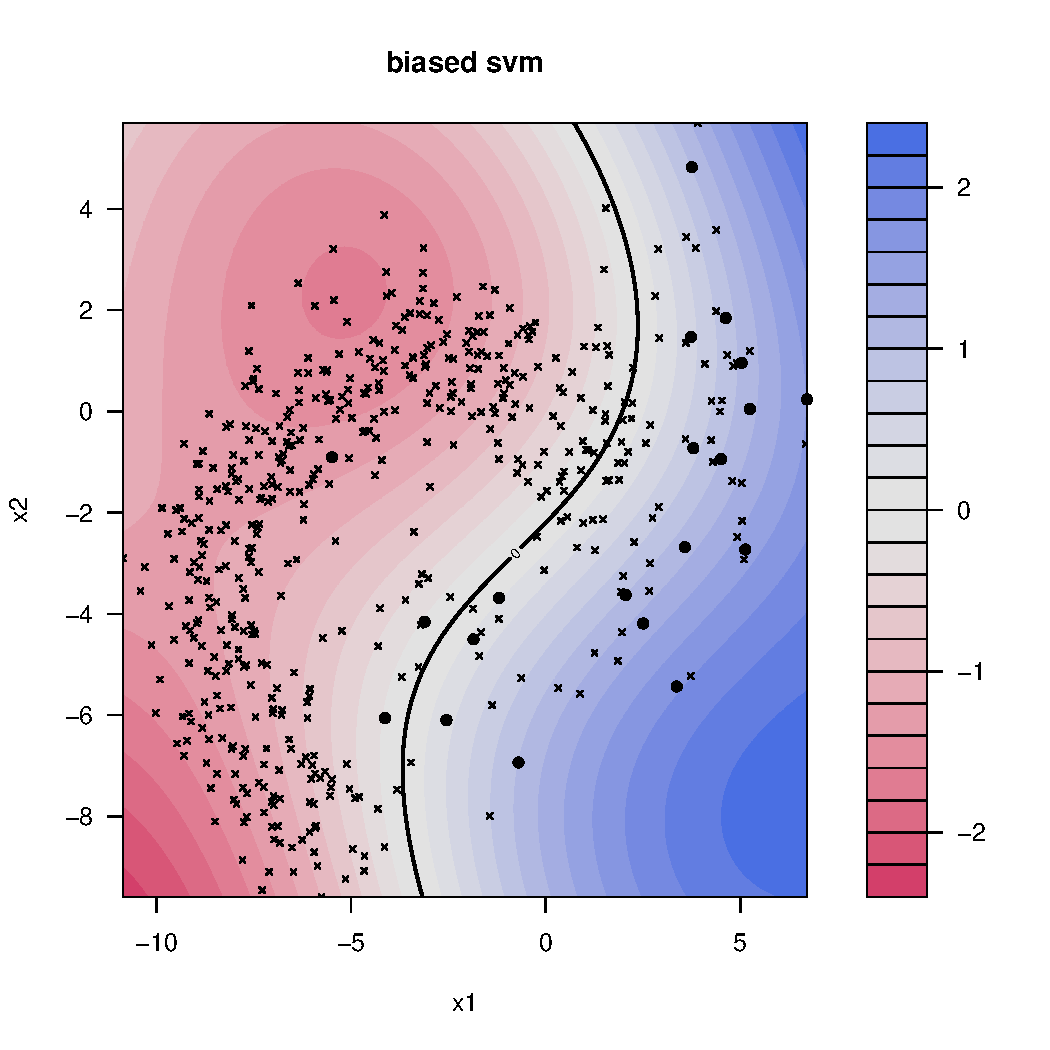
\includegraphics[width=\maxwidth]{figures/plots-update2_fs} 

}



\end{knitrout}

\begin{knitrout}
\definecolor{shadecolor}{rgb}{0.969, 0.969, 0.969}\color{fgcolor}

{\centering 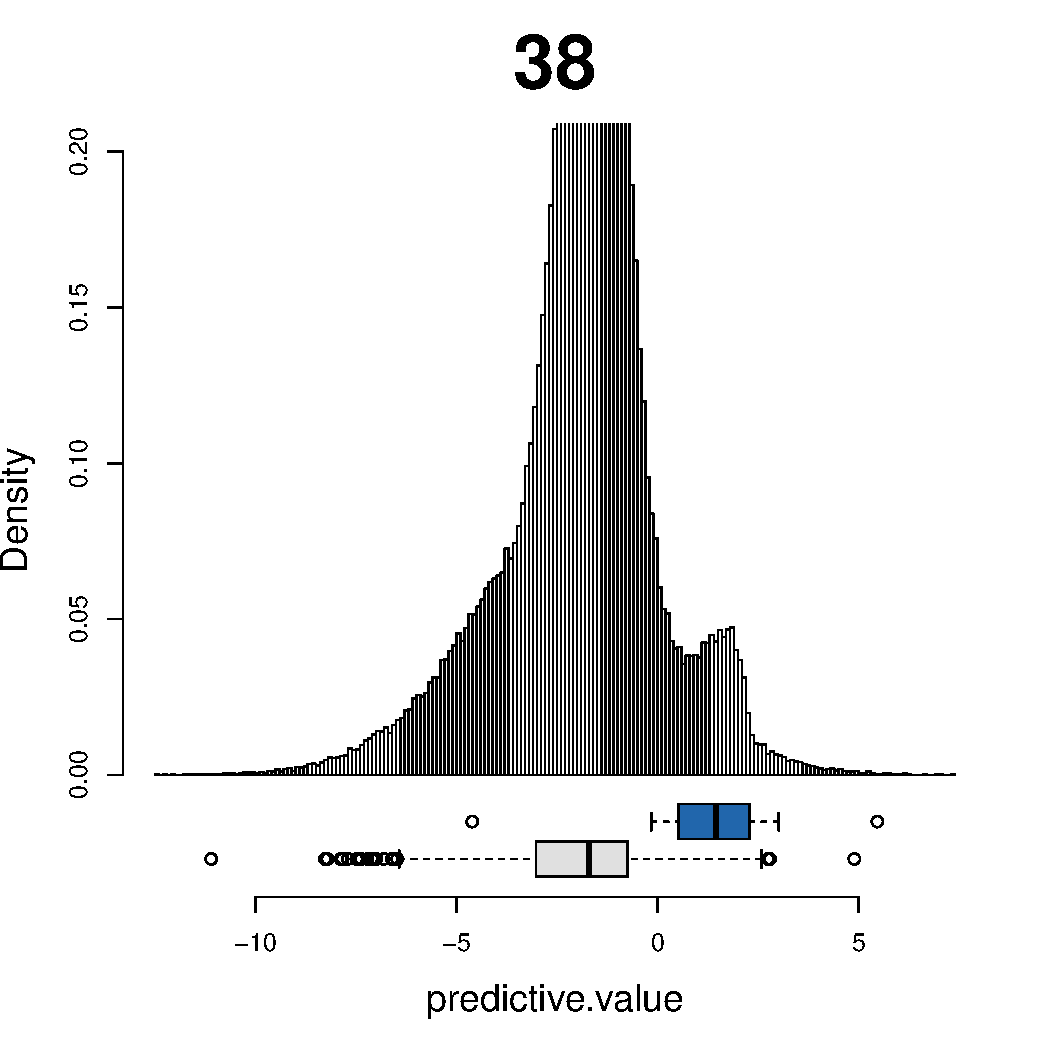
\includegraphics[width=\maxwidth]{figures/plots-update3_hist} 

}



\end{knitrout}

\begin{knitrout}
\definecolor{shadecolor}{rgb}{0.969, 0.969, 0.969}\color{fgcolor}

{\centering 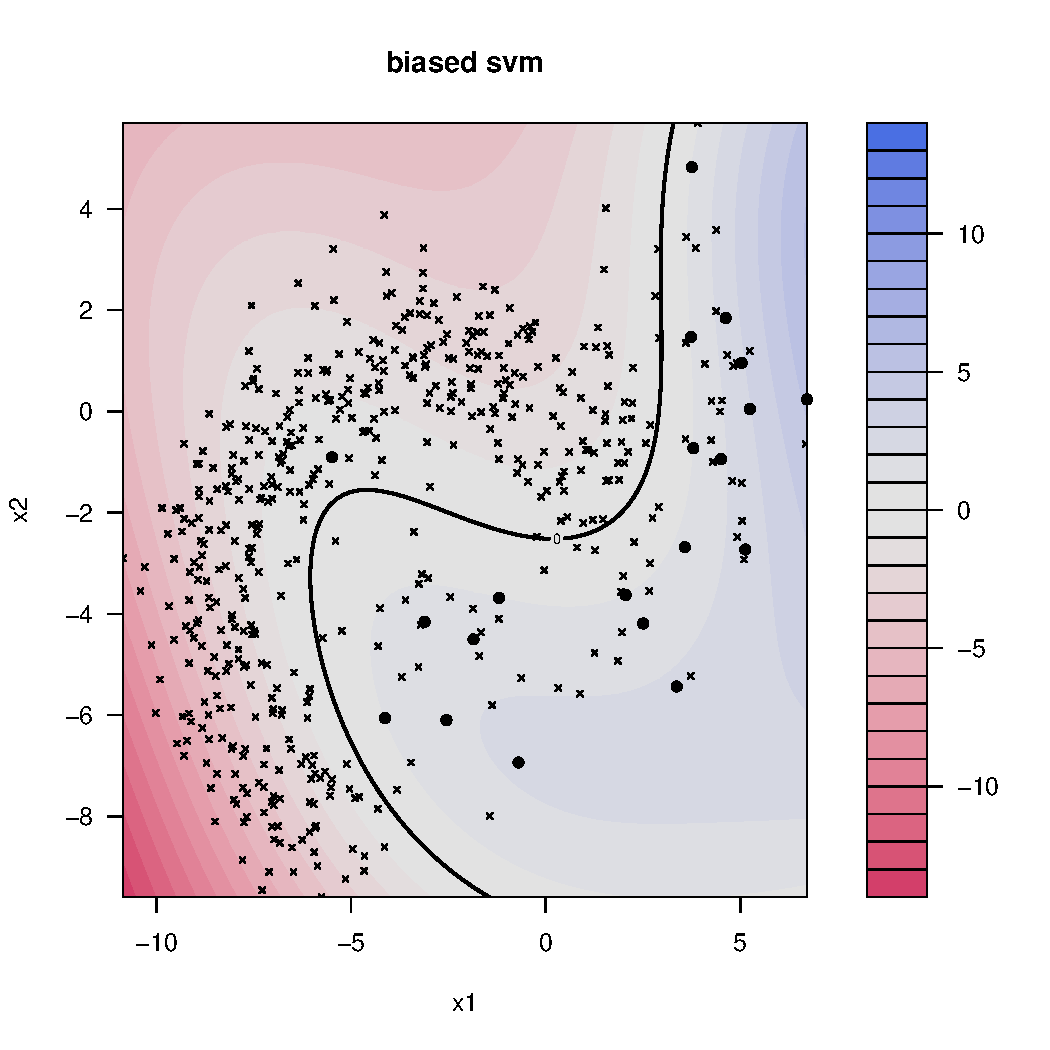
\includegraphics[width=\maxwidth]{figures/plots-update3_fs} 

}



\end{knitrout}

\end{multicols}

Note that the model \#35 (i.e. the model in the 35th row of the \code{oc\$results} data frame) 
is ranked highest in the resamples-plot \note{Find out how the ranking works? Median? Can it be customized?}. 
Second the dagnostic histogram plot shows a clear distinctive data cluster at high predictive values separated by a low density ara from the large part of the data.
From the diagnostic histgram plot we would intuitively identify the one of model \#35 as the one which shows highest discriminative power, or in other words smallest overlapping between the positive and the negative class distributions. 
If we require a binary classification result we would intuitively threshold the predictive outcome at around 0, i.e. somewhere in the separating low density area.

Instead, in model #26 we should expect a higher overlap and it is less trivial to make a decision about a binarization threshold.

\section{Evaluation with PN-data}
\label{sec:evaluation}





In the last section we assumed that no complete and representative test data is avaialble when the model has to be constructed. 
In other situations PN-data might be available and 

However, in other  many situations PN-data is available which makes a traditional accuracy assessment possible.
There are different aspects we might want to evaluate. 
Given a particular model and threshold have been selected the confusion matrix and thereof derived accuracy measures for the binary classification result are of interest.
We can calculate this with the function evaluate:

\begin{knitrout}\footnotesize
\definecolor{shadecolor}{rgb}{0.969, 0.969, 0.969}\color{fgcolor}\begin{kframe}
\begin{alltt}
\hlstd{te.pred} \hlkwb{<-} \hlkwd{predict}\hlstd{(oc, bananas}\hlopt{$}\hlstd{x[te.i])}
\hlstd{ev} \hlkwb{<-} \hlstd{dismo::}\hlkwd{evaluate}\hlstd{(}\hlkwc{p}\hlstd{=te.pred[te.y}\hlopt{==}\hlnum{1}\hlstd{],} \hlkwc{a}\hlstd{=te.pred[te.y}\hlopt{!=}\hlnum{1}\hlstd{])}
\hlstd{ev.th0} \hlkwb{<-} \hlkwd{evaluate}\hlstd{(ev,} \hlkwc{th}\hlstd{=}\hlnum{0}\hlstd{)}
\hlstd{ev.th0}
\end{alltt}
\begin{verbatim}
## Positive/negative (+/-) test samples:
##  105 / 895 
## 
## Confusion Matrix at threshold 0.0084 : 
## 
##           + (Test) - (Test)  SUM UA[%]
## + (Pred)        75       17   92    82
## - (Pred)        30      878  908    97
## SUM            105      895 1000      
## PA[%]           71       98           
## ---                                   
## OA[%]           95                    
## AUC[*100]       97                    
## K[*100]         74
\end{verbatim}
\end{kframe}
\end{knitrout}

If we are interested in the evolution of the accuracy over different thresholds 
we can also specify a vector of threshold or just leave the argument away in which 
case several thresholds are generated automatically over the range of the predictive values.
From this we might also derive maximum achievable accuracy, i.e. the accuracy at the threshold which optimizes a given accuracy metric, e.g. the $\kappa$ coefficient.

\begin{knitrout}
\definecolor{shadecolor}{rgb}{0.969, 0.969, 0.969}\color{fgcolor}\begin{kframe}
\begin{alltt}
\hlkwd{plot}\hlstd{(ev)}
\hlkwd{evaluate}\hlstd{(ev,} \hlkwc{th}\hlstd{=}\hlstr{'max.kappa'}\hlstd{)}
\end{alltt}
\end{kframe}
\end{knitrout}

\begin{multicols}{2}
\begin{knitrout}
\definecolor{shadecolor}{rgb}{0.969, 0.969, 0.969}\color{fgcolor}

{\centering 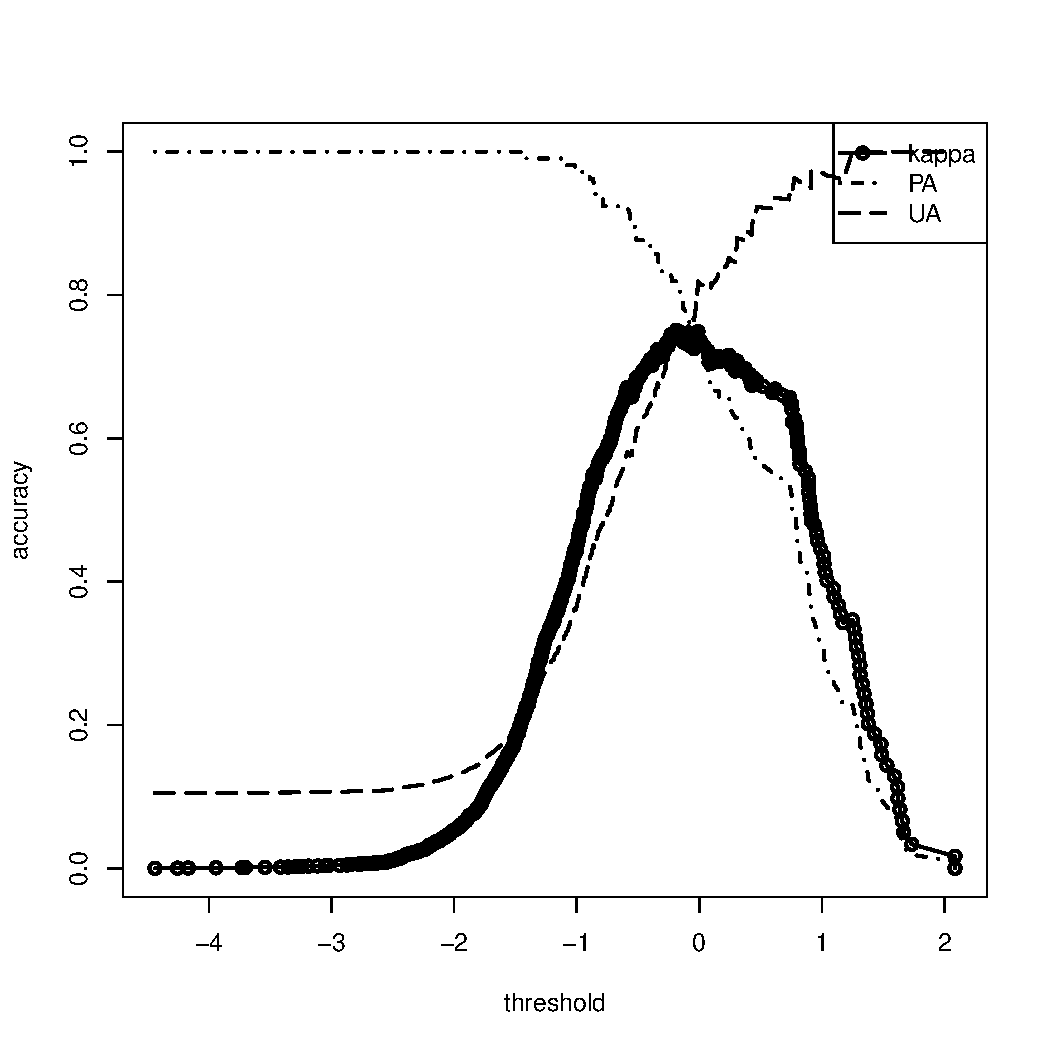
\includegraphics[width=\maxwidth]{figures/plots-evalDepTh_plot} 

}



\end{knitrout}

\begin{knitrout}\footnotesize
\definecolor{shadecolor}{rgb}{0.969, 0.969, 0.969}\color{fgcolor}\begin{kframe}
\begin{verbatim}
## Positive/negative (+/-) test samples:
##  105 / 895 
## 
## Confusion Matrix at threshold -0.1871 : 
## 
##           + (Test) - (Test)  SUM UA[%]
## + (Pred)        86       30  116    74
## - (Pred)        19      865  884    98
## SUM            105      895 1000      
## PA[%]           82       97           
## ---                                   
## OA[%]           95                    
## AUC[*100]       97                    
## K[*100]         75
\end{verbatim}
\end{kframe}
\end{knitrout}
\end{multicols}

Finally, we might also want to evaluate the whole model selection process, e.g. by 
calculating the maximum achievable accuracy for all models.
This can be useful, e.g. to compare differnet model selection approaches, in particular, the performance metrics and/or the resampling approaches to estimate these metrics \note{[REF]}.
Here for example, the best achievable $\kappa$ (y-axis) of each model is plotted against the \code{puF} (x-axis, left plot) and the \code{puAuc} (x-axis, right plot) metric.  

\begin{knitrout}
\definecolor{shadecolor}{rgb}{0.969, 0.969, 0.969}\color{fgcolor}\begin{kframe}
\begin{alltt}
\hlstd{ev.modsel} \hlkwb{<-} \hlkwd{evaluate}\hlstd{(oc,} \hlkwc{y}\hlstd{=te.y,} \hlkwc{u}\hlstd{=te.x,} \hlkwc{allModels}\hlstd{=}\hlnum{TRUE}\hlstd{,} \hlkwc{positive}\hlstd{=}\hlnum{1}\hlstd{)}
\end{alltt}
\end{kframe}
\end{knitrout}

\begin{multicols}{2}
\begin{knitrout}
\definecolor{shadecolor}{rgb}{0.969, 0.969, 0.969}\color{fgcolor}\begin{kframe}
\begin{alltt}
\hlkwd{plot}\hlstd{(ev.modsel,} \hlkwc{fromTrain}\hlstd{=}\hlstr{'puF'}\hlstd{)}
\end{alltt}
\end{kframe}

{\centering 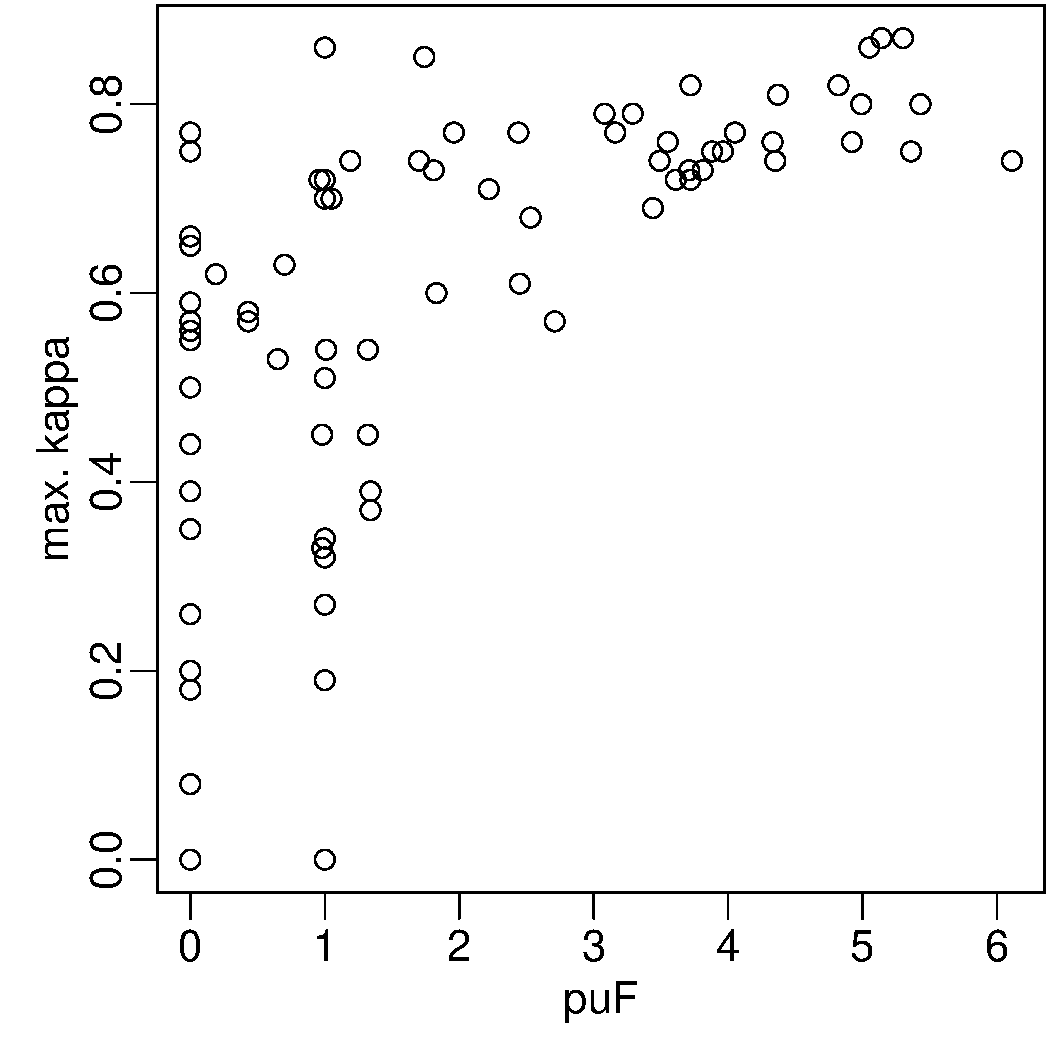
\includegraphics[width=\maxwidth]{figures/plots-evalModsel_puF} 

}



\end{knitrout}

\begin{knitrout}
\definecolor{shadecolor}{rgb}{0.969, 0.969, 0.969}\color{fgcolor}\begin{kframe}
\begin{alltt}
\hlkwd{plot}\hlstd{(ev.modsel,} \hlkwc{fromTrain}\hlstd{=}\hlstr{'puAuc'}\hlstd{)}
\end{alltt}
\end{kframe}

{\centering 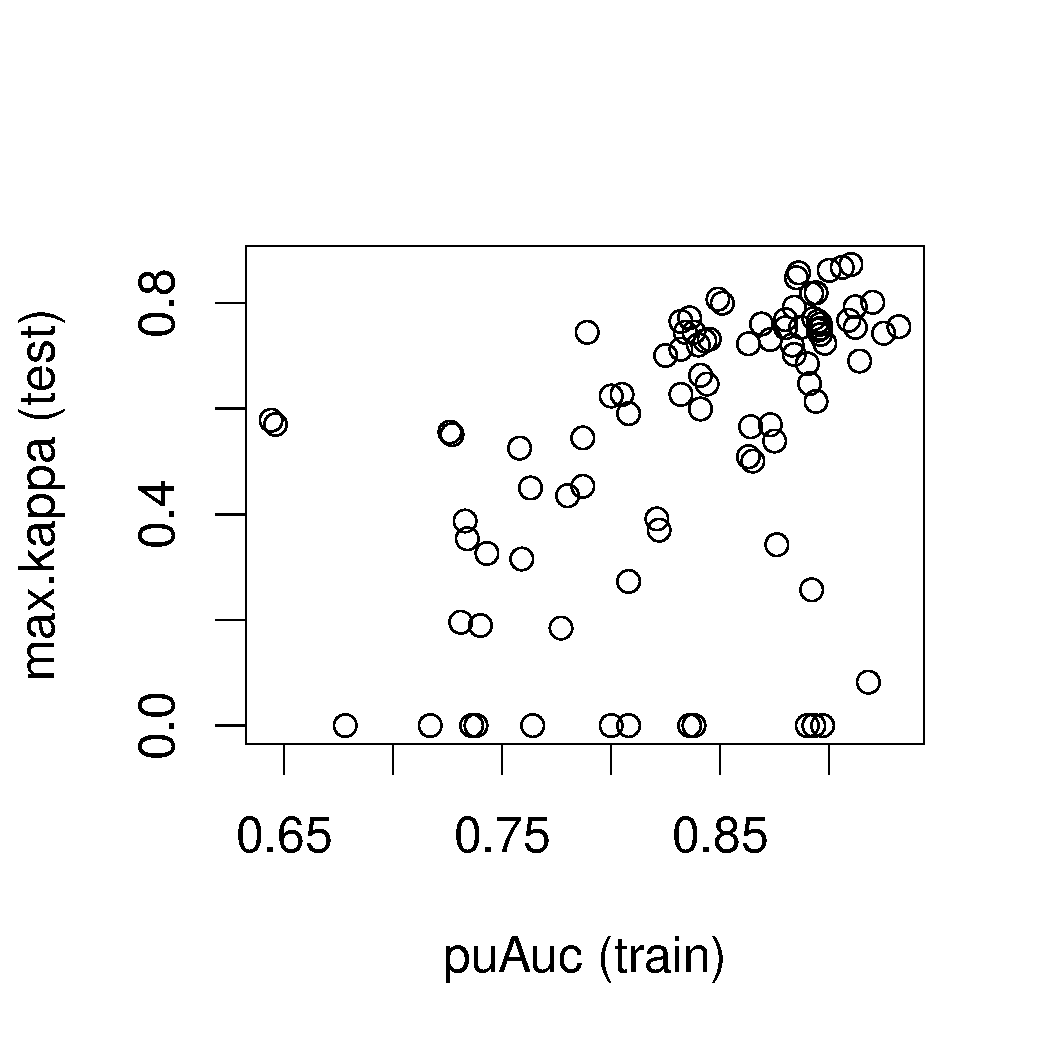
\includegraphics[width=\maxwidth]{figures/plots-evalModsel_puAuc} 

}



\end{knitrout}
\end{multicols}

\section {More one-class classifiers...}
\label{sec:occ}

Currently three classifiers are implemented: the biaseed SVM \cite{Liu.2003} 
and one-class SVM \cite{Scholkopf.2001} 
via the package \hlstd{kernlab} \cite{Karatzoglou.2004}
and maxent \cite{Phillips.2008b} via the package dismo \cite{Hijmans.2013}.

You can see the definition of the interfaces, or custom \hlkwd{train}\hlstd{()} methods, 
with the \hlkwd{getModelInfoOneClass}\hlstd{()}
If you want to use your own one-class classifier with the \hlstd{oneClass}/\hlstd{caret} 
infrastructure you can use these models as examples, but see also the explanations 
on \url{http://caret.r-forge.r-project.org/custom_models.html}.

\section {Parallel processing}
\label{sec:parallel}

Some tasks, e.g. model selection and predictions (see below), can be processed in parallel via the foreach package. 
If you want to use the parallel processing capabilities you need to register a foreach parallel backend.
This can be done as follows:
\begin{knitrout}
\definecolor{shadecolor}{rgb}{0.969, 0.969, 0.969}\color{fgcolor}\begin{kframe}
\begin{alltt}
\hlkwd{require}\hlstd{(foreach)}
\hlkwd{require}\hlstd{(doParallel)}
\hlstd{cl} \hlkwb{<-} \hlkwd{makeCluster}\hlstd{(}\hlkwd{detectCores}\hlstd{()}\hlopt{-}\hlnum{1}\hlstd{)} \hlcom{# leave one core free}
\hlkwd{registerDoParallel}\hlstd{(cl)}
\end{alltt}
\end{kframe}
\end{knitrout}

\section {Prediction of large raster data}
\label{sec:largedata}

If you have large raster files you might want to work with a \Sexexpr('rasterTiled') object. The package can also be downloaded from GitHub \url{https://github.com/benmack/rasterTiled}.
This is a straightforward way of predicting large raster files in parallel. 

The function \hlkwd{rasterTiled}\hlstd{()} returns an S3 object, say \hlstd{rt} which holds
the raster, the valid cells and the start and end indices of the tiles. 

\begin{knitrout}
\definecolor{shadecolor}{rgb}{0.969, 0.969, 0.969}\color{fgcolor}\begin{kframe}
\begin{alltt}
\hlkwd{require}\hlstd{(rasterTiled)}
\end{alltt}


{\ttfamily\noindent\itshape\color{messagecolor}{\#\# Loading required package: rasterTiled}}\begin{alltt}
\hlstd{rt} \hlkwb{<-} \hlkwd{rasterTiled}\hlstd{(bananas}\hlopt{$}\hlstd{x)}
\hlkwd{names}\hlstd{(rt)}
\end{alltt}
\begin{verbatim}
## [1] "raster"     "validCells" "tiles"
\end{verbatim}
\begin{alltt}
\hlstd{rt} \hlcom{# also estimates the approximate size of the tiles in memory}
\end{alltt}
\begin{verbatim}
## class       : RasterBrick 
## dimensions  : 400, 400, 160000, 2  (nrow, ncol, ncell, nlayers)
## resolution  : 1, 1  (x, y)
## extent      : 0, 400, 0, 400  (xmin, xmax, ymin, ymax)
## coord. ref. : NA 
## data source : in memory
## names       :    x1,    x2 
## min values  : -12.6, -11.7 
## max values  : 7.941, 7.188 
## 
## Valid cells: 160000 of 160000.
## 
## Tiles: 
##          tile1 tile2  tile3  tile4
## idxStart     1 5e+04 100001 150001
## idxEnd   50000 1e+05 150000 160000
## 
## Approx. size per tile (Mb):
## 10.3 10.3 10.3 2.1
\end{verbatim}
\end{kframe}
\end{knitrout}

See also the package \Sexexpr{'spatial.tools'} ...

Show an example...

\section {Future work ...}
\label{sec:outlook}

\begin{itemize}
  \item Improve PU-performance metrics
  \item Feature selection
  \item A Posteriori probabilities form the one-class output
  \item Efficient handling of unlabeled data: an iterative approach
  \item Merging one-class classification outputs of different classes
\end{itemize}

\section*{Acknowledgements}
This document was produced in RStudio using the knitr package \cite{knitr2013}.
 
\printbibliography

\end{document}
